\documentclass{beamer}

\beamertemplatenavigationsymbolsempty
\usetheme{Warsaw}

\title{Tic Tac Toe}
\subtitle{Game Design Presentation}
\subject{Tic Tac Toe game design presentation}
\author{James Richey}
\date{February 15, 2020}

% The institute block is convenient for holding
% additional information about the game.
\institute{
  A casual game for all ages\\
  Windows, Linux, and Mac\\
  Coming Summer 2020
}


\begin{document}


\begin{frame}
  \titlepage
\end{frame}


\begin{frame}
  \frametitle{Game Summary}

  \begin{itemize}
    \item Unique take on a classic game
    \item Play in a variety of stunning environments
    \item Single and multiplayer
    \item Free and open source
  \end{itemize}
\end{frame}


\begin{frame}
  \frametitle{Gameplay Overview}

  \begin{itemize}
    \item Players take turns placing their mark in a $3\times3$ gird
    \item First player to get three marks in a row wins
    \item Cat's game occurs if all the free spaces are exhausted
  \end{itemize}

  \begin{figure}
    \vspace{1em}
    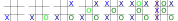
\includegraphics[width=1\textwidth]{img/tic-tac-toe-example-game}
  \end{figure}

\end{frame}


\begin{frame}
  \frametitle{Environments}

  \begin{itemize}
    \item Tells the past, present, and future story of Tic Tac Toe
    \item Strong visual themes and complementary soundtracks
    \item Key differentiation from other Tic Tac Toe games
    \item Over 20 beautiful environments
    \item Each game takes place in a different environment
  \end{itemize}

  \begin{figure}
    \vspace{1em}
    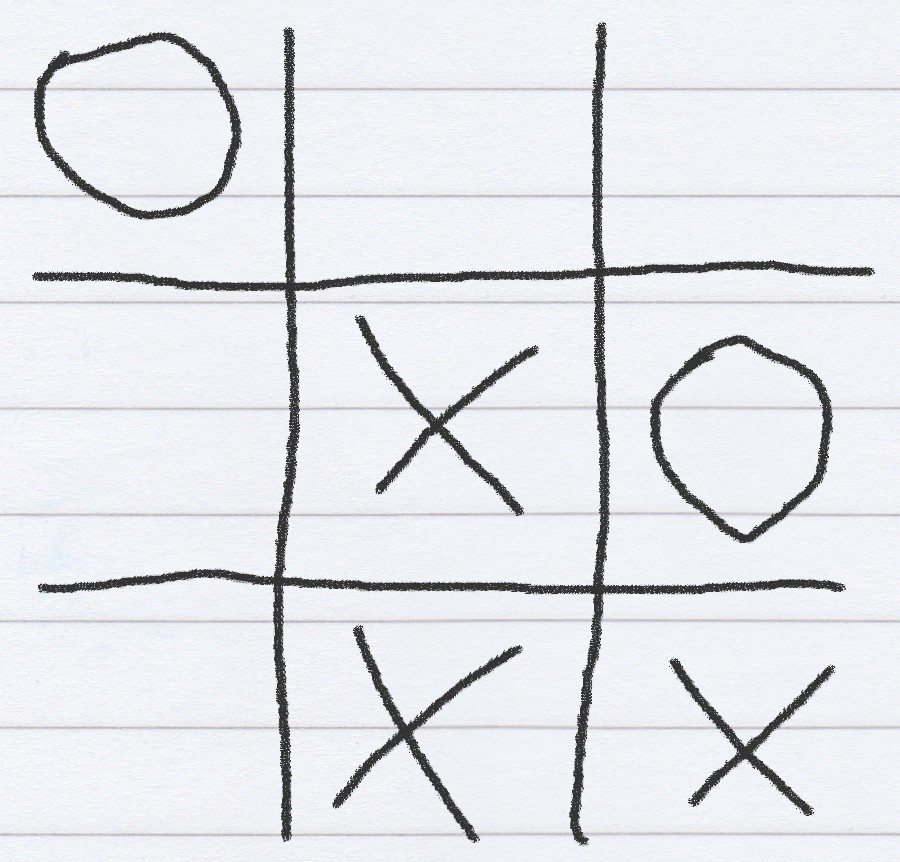
\includegraphics[width=0.24\textwidth]{img/concept-art/paper}
    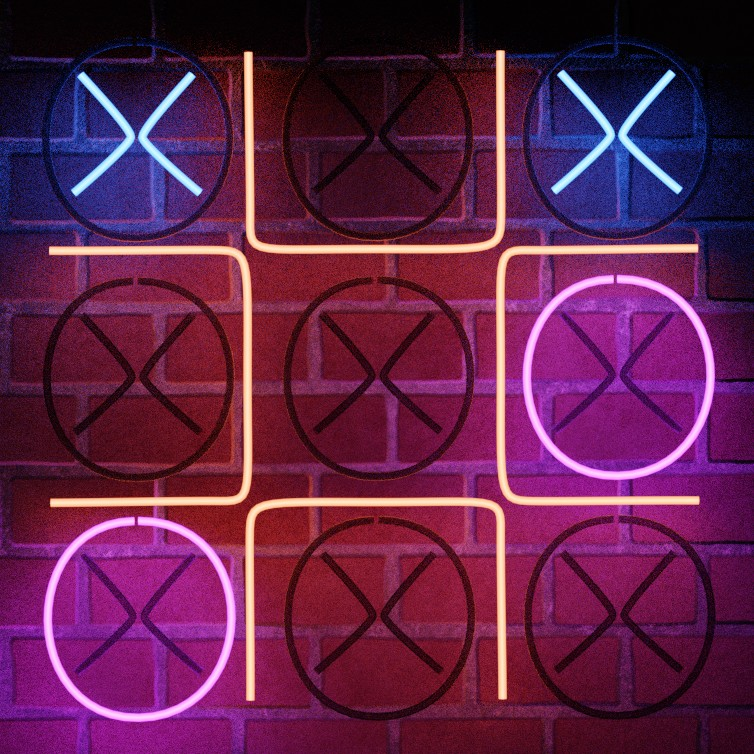
\includegraphics[width=0.24\textwidth]{img/concept-art/neon}
    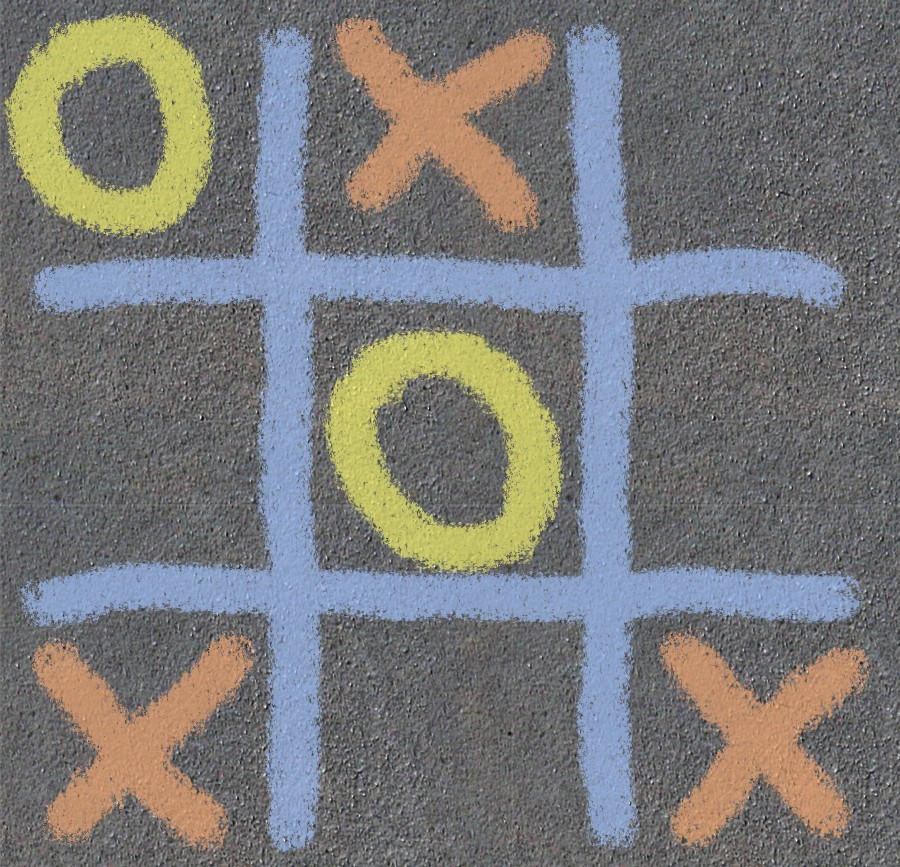
\includegraphics[width=0.24\textwidth]{img/concept-art/sidewalk}
    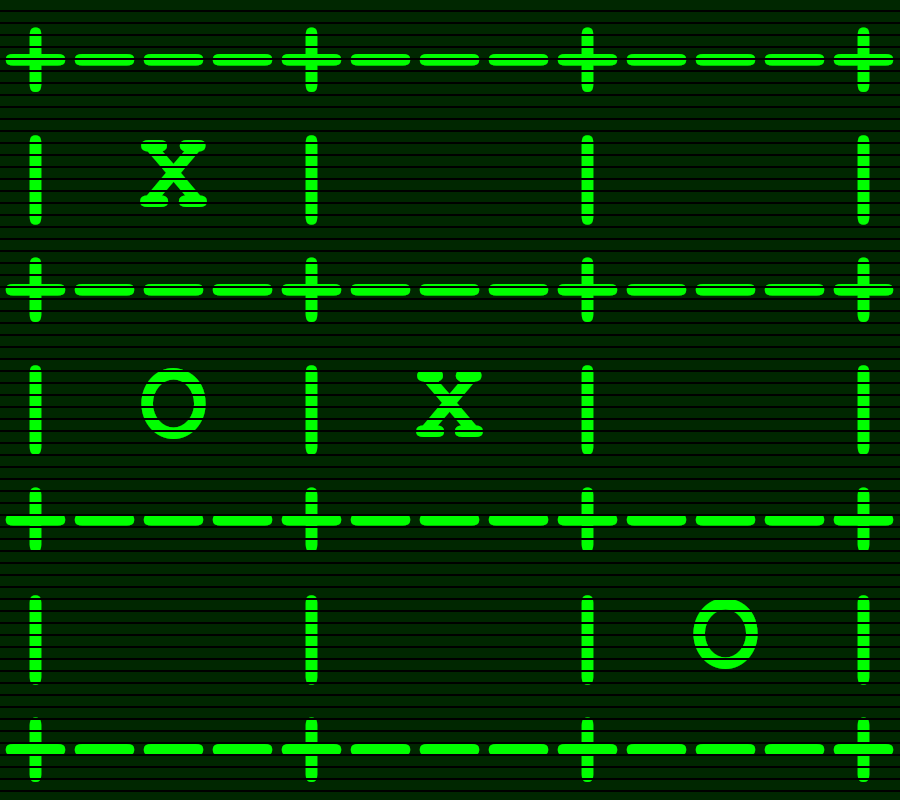
\includegraphics[width=0.24\textwidth]{img/concept-art/computer}
  \end{figure}

\end{frame}


\begin{frame}
  \frametitle{Controls}

  \begin{itemize}
    \item Keyboard and mouse
    \item Select squares with left click or the numpad
    \item Escape to open the game's menu
    \item Access game options and credits from game's menu
  \end{itemize}

  \begin{figure}
    \vspace{1em}
    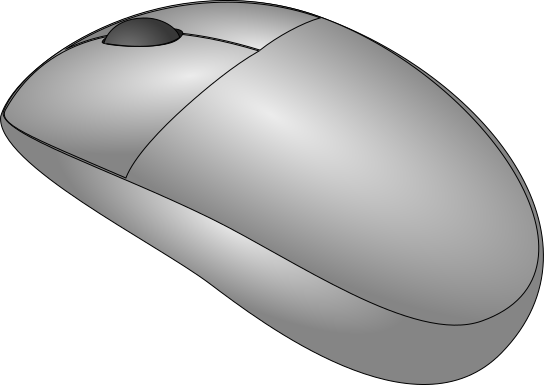
\includegraphics[width=0.4\textwidth]{img/clip-art/computer-mouse}
  \end{figure}

\end{frame}


\begin{frame}
  \frametitle{Monetization}

  \begin{itemize}
    \item Free
    \item Open source with code hosted on GitHub
    \item No advertisements or tracking
  \end{itemize}

  \begin{figure}
    \vspace{1em}
    
\includegraphics[height=0.40\textheight]{img/clip-art/no-money}
  \end{figure}

\end{frame}


\begin{frame}
  \frametitle{Production}

  \begin{itemize}
    \item Programmed using Rust, Piston, and open\_ttt\_lib
    \item Make prototype to reduce risk
    \item Launch Summer 2020
    \item Additional environments added in future releases
  \end{itemize}

  \begin{figure}
    \vspace{1em}
    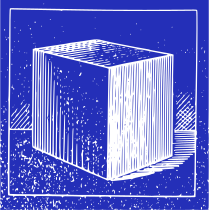
\includegraphics[height=0.40\textheight]{img/clip-art/blueprint-cube}
  \end{figure}

\end{frame}


\begin{frame}
  \frametitle{Questions}

  \begin{figure}
    
\includegraphics[height=0.50\textheight]{img/clip-art/question-mark}
  \end{figure}

\end{frame}


\end{document}
